\section{分布优化问题}
\label{sec:dsel-problems}

章首的三种愿望听起来都合理，可它们在数学上扮演的角色不同：有的是要尽量减小的量，有的是必须满足的等式，有的是不愿付出的代价。在写任何公式之前，先把它们在同一个小例子里分别算清楚，再规定一个分布优化问题由哪些部分组成。

\paragraph{三种不同的要求}
取$\mathcal{X}=\{0,1,2\}$，参考分布$P$是均匀分布，三个概率都是$1/3$。待选的分布$Q$由三个数$q(0),q(1),q(2)$给出，它们非负且和为$1$，全体这样的$Q$构成第~\ref{chap:distribution-families}章的概率三角形，三个顶点是单点分布$\delta_0,\delta_1,\delta_2$。设每个状态有一个成本$V(x)=x$。

第一种要求是降低期望成本。期望成本
\[
 \mathbb{E}_{Q}[V]=q(1)+2q(2)
\]
是$Q$的线性函数，它在三角形上的等值线是一族平行线。线性函数在三角形上的最小值一定在某个顶点取到，这里是$\delta_0$，最小值为$0$。这个答案把原本可能的状态$1$和$2$全部删掉了。若两个状态的成本相同且都最小，例如$V(0)=V(1)=0$，那么整条边上的分布都同样好，答案也不唯一。

第二种要求是满足指定的平均量，例如$\mathbb{E}_{Q}[X]=10/7$。它和归一化一起是三个未知数的两个线性方程：
\[
 q(1)+2q(2)=\frac{10}{7},\qquad q(0)+q(1)+q(2)=1 .
\]
令$q(1)=0$，解得$q(2)=5/7$，$q(0)=2/7$；令$q(0)=0$，解得$q(2)=3/7$，$q(1)=4/7$。满足要求的分布是连接$(\tfrac27,0,\tfrac57)$与$(0,\tfrac47,\tfrac37)$的一条线段，有无穷多个。约束本身不能从中挑出一个。

第三种要求是接近参考分布。用第~\ref{chap:distribution-comparison}章的KL散度衡量偏离，$D_{\mathrm{KL}}(Q\Vert P)\geq0$，且等号当且仅当$Q=P$。只最小化它，得到的就是$P$本身，什么也没有改变。

图~\ref{fig:dsel-three-requirements}把三种要求画在同一个三角形里。成本的等值线与平均量的约束线方向相同，因为这里成本和约束用的是同一个函数$x$，红色线段也就是期望成本等于$10/7$的那条等值线。只有把它们组合起来，例如“在红线上找离$P$最近的点”，问题才既不平凡又有确定的答案。

\begin{BookInlineFigure}
 \centering
 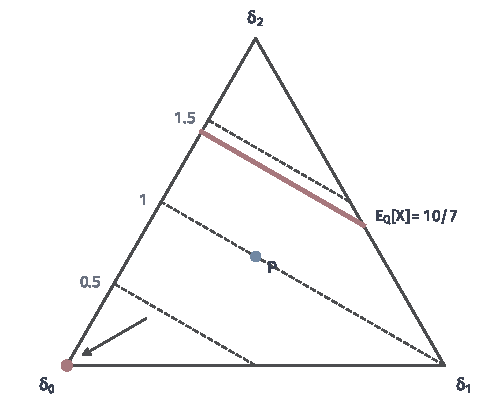
\includegraphics[width=84mm]{figures/07-probability/07-distribution-optimization/matplotlib/dsel-three-requirements/figure.pdf}
 \caption{$\{0,1,2\}$上的三种要求。三角形中每一点是一张概率表。深灰虚线是期望成本$\mathbb{E}_{Q}[V]=q(1)+2q(2)$的等值线，标注为取值，箭头指向成本最小的顶点$\delta_0$（红点）；红色线段是满足$\mathbb{E}_{Q}[X]=10/7$的全部分布；蓝点是参考分布$P$。}
 \label{fig:dsel-three-requirements}
\end{BookInlineFigure}

本章研究的三类问题正是这样的组合：
\begin{enumerate}
 \item 不加等式约束，最小化期望成本加上偏离参考分布的代价$\tau D_{\mathrm{KL}}(Q\Vert P)$，$\tau>0$调节两者的比重；
 \item 要求$\mathbb{E}_{Q}[\bm{T}]=\bm{m}$，在满足要求的分布中最小化$D_{\mathrm{KL}}(Q\Vert P)$；
 \item 要求$\mathbb{E}_{Q}[\bm{T}]=\bm{m}$，在满足要求的分布中最大化熵。
\end{enumerate}
其中$\bm{T}:\mathcal{X}\to\mathbb{R}^{k}$是若干个指定的统计量，$\bm{m}\in\mathbb{R}^{k}$是它们的指定平均值。

\paragraph{允许的分布}
一般情形下，$\mathcal{X}$是可测空间，记其上全体概率测度为$\mathcal{P}(\mathcal{X})$。待选对象是$\mathcal{P}(\mathcal{X})$中的元素，但并非每个元素都能参加比较。候选集合$\mathcal{Q}\subseteq\mathcal{P}(\mathcal{X})$是问题的一部分，要逐项写明。

非负性与归一化看起来理所当然，计算时却最容易丢掉。在上面的例子里，若只解那两个线性方程，以$q(1)=t$为参数，得到
\[
 q(2)=\frac57-\frac t2,\qquad q(0)=\frac27-\frac t2 .
\]
取$t=1$，得到$(-\tfrac{3}{14},1,\tfrac{3}{14})$。它和为$1$，平均值也是$10/7$，但$q(0)<0$，不是概率表。只有$0\leq t\leq4/7$才合法。凡是用方程、公式或数值迭代得出的“分布”，都要回头核对这两条。

其次是支持。若$Q$在$P$概率为零的地方放了质量，即$Q$不绝对连续于$P$，则$D_{\mathrm{KL}}(Q\Vert P)=+\infty$。所以只要目标里含有$D_{\mathrm{KL}}(Q\Vert P)$，有意义的候选都满足$Q\ll P$：选出的分布可以删去参考分布的状态，但不能添加新的状态。

最后是可积性。期望成本$\mathbb{E}_{Q}[V]$与约束中的$\mathbb{E}_{Q}[\bm{T}]$都要求相应函数在$Q$下可积，否则目标或约束不是一个确定的实数。有限状态上这一条自动成立，可数或连续状态上必须单独检查。

\begin{definition}[分布优化问题]
\label{def:dsel-problem}
设$\mathcal{Q}\subseteq\mathcal{P}(\mathcal{X})$是候选集合，$J:\mathcal{Q}\to(-\infty,+\infty]$。称
\begin{equation}
 J^{*}=\inf_{Q\in\mathcal{Q}}J(Q)
 \label{eq:dsel-problem}
\end{equation}
为\term{分布优化问题}（distribution optimization problem）的最优值。若$Q^{*}\in\mathcal{Q}$满足$J(Q^{*})=J^{*}$，称$Q^{*}$为\term{最优分布}（optimal distribution）。
\end{definition}

定义把三件事分开了。$\mathcal{Q}$非空且$J$在其上有定义，问题才成立；$J^{*}$可能是有限数，也可能是$-\infty$；即使$J^{*}$有限，也可能没有任何$Q$达到它。这三件事在第~\ref{sec:dsel-checks}节逐一检查，这里先看第一件事为什么不能省略。

\paragraph{无穷量不能相减}
目标$\mathbb{E}_{Q}[V]+\tau D_{\mathrm{KL}}(Q\Vert P)$由两项相加。第二项总在$[0,+\infty]$中；第一项若不加限制，可以是$-\infty$。下面的例子中两项分别是$-\infty$和$+\infty$。取$\mathcal{X}=\{1,2,\dots\}$，参考分布与成本为
\[
 P(k)=2^{-k},\qquad V(k)=-k ,
\]
候选分布取$Q(k)=\dfrac{6}{\pi^{2}k^{2}}$。

期望成本是调和级数乘以负数：
\[
 \mathbb{E}_{Q}[V]=-\frac{6}{\pi^{2}}\sum_{k\geq1}\frac1k=-\infty .
\]
再看对数比。对每个$k$，
\[
 \ln\frac{Q(k)}{P(k)}=\ln\frac{6}{\pi^{2}}-2\ln k+k\ln2 .
\]
按$Q$平均时，前两项给出收敛级数，因为$\sum_k(\ln k)/k^{2}<\infty$；第三项给出$\ln2\sum_kkQ(k)=+\infty$。所以$D_{\mathrm{KL}}(Q\Vert P)=+\infty$，目标成了“$-\infty+\infty$”。

把两个级数逐项配对，似乎能得到一个有限数。取$\tau=1/\ln2$，记前$N$项的部分和为
\[
 C_N=\sum_{k\leq N}Q(k)V(k),\qquad K_N=\tau\sum_{k\leq N}Q(k)\ln\frac{Q(k)}{P(k)} .
\]
这时$\tau k\ln2=k$，与$V(k)=-k$恰好抵消，$C_N+K_N$收敛到约$-2.363$。但若把$C_N$与$K_{2N}$配对，多出的部分是$\frac{6}{\pi^{2}}\sum_{N<k\leq2N}\frac1k$，它趋于$\frac{6}{\pi^{2}}\ln2\approx0.421$，极限变成约$-1.941$。图~\ref{fig:dsel-undefined-objective}画出了这几条部分和曲线。

\begin{BookInlineFigure}
 \centering
 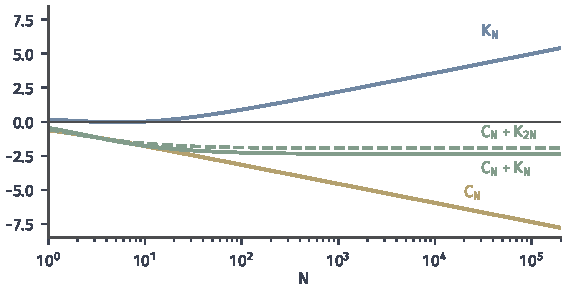
\includegraphics[width=96mm]{figures/07-probability/07-distribution-optimization/matplotlib/dsel-undefined-objective/figure.pdf}
 \caption{无定义的目标。$P(k)=2^{-k}$，$V(k)=-k$，$Q(k)=6/(\pi^{2}k^{2})$，$\tau=1/\ln2$，横轴为对数刻度。黄线是期望成本的部分和$C_N\to-\infty$，蓝线是KL项的部分和$K_N\to+\infty$；绿色实线$C_N+K_N$与绿色虚线$C_N+K_{2N}$各自收敛，极限相差$\frac{6}{\pi^{2}}\ln2\approx0.421$。}
 \label{fig:dsel-undefined-objective}
\end{BookInlineFigure}

一个数值若取决于怎样配对两条发散级数，它就不是目标函数的值。所以凡是目标含$\mathbb{E}_{Q}[V]+\tau D_{\mathrm{KL}}(Q\Vert P)$的问题，本章都把候选集合取为
\begin{equation}
 \mathcal{Q}_V=\Bigl\{Q\in\mathcal{P}(\mathcal{X}):\ D_{\mathrm{KL}}(Q\Vert P)<\infty,\ \mathbb{E}_{Q}\lvert V\rvert<\infty\Bigr\}.
 \label{eq:dsel-candidate-set}
\end{equation}
在$\mathcal{Q}_V$上两项都是有限实数，和有确定的值。有限状态且$P$处处为正时，$\mathcal{Q}_V$就是全部概率表。
